\documentclass[11pt,]{article}
\usepackage{lmodern}
\usepackage{amssymb,amsmath}
\usepackage{ifxetex,ifluatex}
\usepackage{fixltx2e} % provides \textsubscript
\ifnum 0\ifxetex 1\fi\ifluatex 1\fi=0 % if pdftex
  \usepackage[T1]{fontenc}
  \usepackage[utf8]{inputenc}
\else % if luatex or xelatex
  \ifxetex
    \usepackage{mathspec}
  \else
    \usepackage{fontspec}
  \fi
  \defaultfontfeatures{Ligatures=TeX,Scale=MatchLowercase}
\fi
% use upquote if available, for straight quotes in verbatim environments
\IfFileExists{upquote.sty}{\usepackage{upquote}}{}
% use microtype if available
\IfFileExists{microtype.sty}{%
\usepackage{microtype}
\UseMicrotypeSet[protrusion]{basicmath} % disable protrusion for tt fonts
}{}
\usepackage[margin=1.0in]{geometry}
\usepackage{hyperref}
\hypersetup{unicode=true,
            pdfborder={0 0 0},
            breaklinks=true}
\urlstyle{same}  % don't use monospace font for urls
\usepackage{graphicx,grffile}
\makeatletter
\def\maxwidth{\ifdim\Gin@nat@width>\linewidth\linewidth\else\Gin@nat@width\fi}
\def\maxheight{\ifdim\Gin@nat@height>\textheight\textheight\else\Gin@nat@height\fi}
\makeatother
% Scale images if necessary, so that they will not overflow the page
% margins by default, and it is still possible to overwrite the defaults
% using explicit options in \includegraphics[width, height, ...]{}
\setkeys{Gin}{width=\maxwidth,height=\maxheight,keepaspectratio}
\IfFileExists{parskip.sty}{%
\usepackage{parskip}
}{% else
\setlength{\parindent}{0pt}
\setlength{\parskip}{6pt plus 2pt minus 1pt}
}
\setlength{\emergencystretch}{3em}  % prevent overfull lines
\providecommand{\tightlist}{%
  \setlength{\itemsep}{0pt}\setlength{\parskip}{0pt}}
\setcounter{secnumdepth}{0}
% Redefines (sub)paragraphs to behave more like sections
\ifx\paragraph\undefined\else
\let\oldparagraph\paragraph
\renewcommand{\paragraph}[1]{\oldparagraph{#1}\mbox{}}
\fi
\ifx\subparagraph\undefined\else
\let\oldsubparagraph\subparagraph
\renewcommand{\subparagraph}[1]{\oldsubparagraph{#1}\mbox{}}
\fi

%%% Use protect on footnotes to avoid problems with footnotes in titles
\let\rmarkdownfootnote\footnote%
\def\footnote{\protect\rmarkdownfootnote}

%%% Change title format to be more compact
\usepackage{titling}

% Create subtitle command for use in maketitle
\newcommand{\subtitle}[1]{
  \posttitle{
    \begin{center}\large#1\end{center}
    }
}

\setlength{\droptitle}{-2em}

  \title{}
    \pretitle{\vspace{\droptitle}}
  \posttitle{}
    \author{}
    \preauthor{}\postauthor{}
    \date{}
    \predate{}\postdate{}
  
\usepackage{helvet} % Helvetica font
\renewcommand*\familydefault{\sfdefault} % Use the sans serif version of the font
\usepackage[T1]{fontenc}

\usepackage[none]{hyphenat}

\usepackage{setspace}
\doublespacing
\setlength{\parskip}{1em}

\usepackage{lineno}

\usepackage{pdfpages}

\begin{document}

\vspace{35mm}

\section{\texorpdfstring{The proton pump inhibitor omeprazole does not
promote \emph{Clostridium difficile} colonization in a murine
model}{The proton pump inhibitor omeprazole does not promote Clostridium difficile colonization in a murine model}}\label{the-proton-pump-inhibitor-omeprazole-does-not-promote-clostridium-difficile-colonization-in-a-murine-model}

\vspace{35mm}

Sarah Tomkovich\({^1}\), Nicholas A. Lesniak\({^1}\), Yuan Li\({^1}\),
Lucas Bishop\({^1}\), Madison J. Fitzgerald\({^1}\), Patrick D.
Schloss\textsuperscript{1\(\dagger\)}

\vspace{40mm}

\(\dagger\) To whom correspondence should be addressed:
\href{mailto:pschloss@umich.edu}{\nolinkurl{pschloss@umich.edu}}

\(1\) Department of Microbiology and Immunology, University of Michigan,
Ann Arbor, MI 48109

\newpage

\linenumbers

\subsection{Abstract}\label{abstract}

Proton pump inhibitor (PPI) use has been associated with microbiota
alterations and susceptibility to \emph{Clostridium difficile}
infections (CDIs) in humans. We assessed how PPI treatment alters the
fecal microbiota and whether treatment promotes CDIs in a mouse model.
Mice receiving a PPI treatment were gavaged with 40 mg/kg of omeprazole
during a 7-day pretreatment phase, the day of \emph{C. difficile}
challenge, and the following 9 days. We found that mice treated with
omeprazole were not colonized by \emph{C. difficile}. When omeprazole
treatment was combined with a single clindamycin treatment, one cage of
mice remained resistant to \emph{C. difficile} colonization, while the
other cage was colonized. Treating mice with only clindamycin followed
by challenge resulted in \emph{C. difficile} colonization. 16S rRNA gene
sequencing analysis revealed that omeprazole had minimal impact on the
structure of the murine microbiota throughout the 16 days of omeprazole
exposure. These results suggest omeprazole treatment alone is not
sufficient to disrupt microbiota resistance to \emph{C. difficle}
infection in mice that are normally resistant in the absence of
antibiotic treatment.

\subsection{Importance}\label{importance}

Antibiotics are the primary risk factor for \emph{Clostridium difficile}
infections (CDIs), but other factors may also increase a person's risk.
In epidemiological studies, PPI use has been associated with CDI
incidence and recurrence. Proton pump inhibitors (PPIs) have also been
associated with alterations in the human intestinal microbiota in
observational and interventional studies. We evaluated the effects of
the PPI omeprazole on the structure of the murine intestinal microbiota
and its ability to disrupt colonization resistance to \emph{C.
difficile}. We found omeprazole treatment had minimal impact on the
murine fecal microbiota and did not promote \emph{C. difficile}
colonization. Further studies are needed to determine whether other
factors such as the composition of the starting bacterial community,
comorbidities, and use of additional medications contribute to the
association between PPIs and CDIs seen in humans or whether aspects of
murine physiology may limit its utility to test these types of
hypotheses.

\newpage

Antibiotics have a large impact on the intestinal microbiome and are a
primary risk factor for developing \emph{Clostridium difficile}
infections (CDIs) (1). It is less clear whether other human medications
that impact the microbiota also influence \emph{C. difficile}
colonization resistance. Multiple epidemiological studies have suggested
an association between proton pump inhibitor (PPI) use and incidence or
recurrence of CDIs (2--5). There have also been a number of large cohort
studies and interventional clinical trials that demonstrated specific
alterations in the intestinal microbiome were associated with PPI use
(4, 6). PPI-associated microbiota changes have been attributed to the
ability of PPIs to increase stomach acid pH which may promote the
survival of oral and pathogenic bacteria (4, 6). In human fecal samples,
PPI use results in increases in Enterococcaceae, Lactobacillaceae,
Micrococcaceae, Staphylococcaceae and Streptococcaceae and decreases in
Ruminococcaceae (6--9). Several of these taxa have also been associated
with \emph{C. difficile} colonization in humans (10).\\
Unfortunately, most of the studies suggesting a link between PPIs and
\emph{C. difficile} were retrospective and did not evaluate changes in
the microbiome (2, 3, 5). Thus, it is unclear whether the
gastrointestinal microbiome changes associated with PPI use explain the
association between PPIs and CDIs. Additionally, epidemiological studies
have a limited capacity to address potential confounders and
comorbidities in patients that were on PPIs and developed CDIs or
recurrent CDIs (2, 5). Here, we evaluated the impact of daily PPI
treatment with omeprazole on the murine microbiome and susceptibility to
\emph{C. difficile} colonization in relation to clindamycin, an
antibiotic that perturbs the microbiome enough to allow \emph{C.
difficile} to colonize but is mild enough that \emph{C. difficile} is
cleared within 10 days (11).

\textbf{Murine fecal microbiomes were minimally affected by omeprazole
treatment } To test whether omeprazole treatment alters the microbiome
and promotes susceptibility to CDIs, we gavaged mice with 40 mg/kg of
omeprazole for 7 days before \emph{C. difficile} challenge (Figure 1A).
A principle coordinates analysis (PCoA) of the Bray-Curtis distances
over the initial 7 days of treatment revealed the bacterial communities
of omeprazole-treated mice remained relatively unchanged (Figure 1B). We
observed no significant fluctuations in the relative abundance of those
taxa previously shown to respond to PPI treatment throughout the course
of the 16-day experiment (Figure 1C-D, S1). We also observed no
significant changes in relative abundances at the family and genus level
over the course of the experiment for the omeprazole-treated mice (data
not shown). These results demonstrated that the omeprazole treatment
alone had a minimal impact on the murine fecal bacterial community after
7 days of pretreatment.

\textbf{Omeprazole treatment did not promote susceptibility to \emph{C.
difficile infection} in mice} Next, we examined whether omeprazole
treatment altered susceptibility to \emph{C. difficile} infection in
mice. After omeprazole treatment or clindamycin treatment, mice were
challenged with 10\textsuperscript{3} \emph{C. difficile} 630 spores.
While \emph{C. difficile} colonized the clindamycin-treated mice, it did
not colonize the omeprazole-treated mice (Figure 2A). Interestingly,
only 1 cage of mice that received both omeprazole and clindamycin were
colonized, while the other cage of mice were resistant (Figure 2A). The
greatest shifts in bacterial communities occurred in the
clindamycin-treated mice (Figure 2B, S2). Regardless of whether the mice
became colonized, all of the mice had cleared \emph{C. difficile} within
5 days (Figure 2A), suggesting that omeprazole did not affect the rate
of clearance. Our results suggest that omeprazole treatment had no
effect on bacterial community resistance to \emph{C. difficile}
colonization in mice. Instead most of the differences between the 3
treatment groups appeared to be driven by clindamycin administration
(Figure 2C, S2). These findings demonstrated that high dose omeprazole
treatment did not promote susceptibility to \emph{C. difficile}
colonization.

\subsection{Conclusions}\label{conclusions}

We found the PPI omeprazole did not impact the gut microbiota and did
not promote \emph{C. difficile} infection in mice. Our findings that
omeprazole treatment had minimal impact on the fecal microbiome were
comparable to another PPI mouse study that indicated the PPI
lansoprazole had more of an effect on the small intestinal microbiota
compared to the fecal microbiota (12). The same group demonstrated
lansoprazole treatment increased the stomach pH in mice (12), which may
improve survival of bacteria passing through the stomach. We did not
find significant changes for the taxa observed to be significantly
impacted by PPI use in human studies. However, 3 of the human-associated
taxa were absent or at low abundance in our mice. Although our fecal
microbiota findings are comparable to what has been shown in another
mouse study (12), whether PPI-induced changes in specific bacterial
abundances observed in humans play a role in CDIs remains to be
determined.\\
While several \emph{C. difficile} mouse model studies have shown that
PPIs have an effect on CDIs with or without additional antibiotic
treatment (13--15), there were insufficient controls to attribute the
effect solely to PPI treatment. One group administered 0.5 mg/kg of the
PPI lansoprazole daily for 2 weeks to mice and then challenged with
\emph{C. difficile} demonstrated that PPI treatment alone resulted in
detectable \emph{C. difficile} in the stool 1 week after challenge,
however there was detectable \emph{C. difficile} in mice not treated
with antibiotics (13, 14). The other mouse study demonstrated the
antibiotic/PPI (esomeprazole)-treated mice developed more severe CDIs
compared to antibiotic-treated mice, but did not have a group treated
with just esomeprazole for comparison (15). We tested the same high 40
mg/kg PPI dose and expanded pre-treatment to 7 days before challenge to
test the impact of omeprazole treatment alone on our CDI mouse model.
Additionally, we've previously demonstrated that mice from our colony
were resistant to \emph{C. difficile} 630 colonization without
antibiotic treatment (16), ensuring there was not already partial
susceptiblity to \emph{C. difficile} before treatment. The additional
controls in our study allowed us to assess the contibution of omeprazole
alone to \emph{C. difficile} susceptibility in mice.\\
Our study also extended previous work examining PPIs and \emph{C.
difficile} in mice by incorporating the contribution of the intestinal
microbiota. We found the PPI omeprazole had no significant impact on
bacterial taxa within the murine intestinal microbiota over the 16-day
experiment. In contrast to previous work, omeprazole did not alter
\emph{C. difficile} colonization resistance. 16S rRNA sequencing
suggested that \emph{Streptococcus} and \emph{Enterococcus} are rare
genera in our C57BL/6 mouse colony and variation in these 2 genera have
been observed across other facilities and vendors (17, 18). These genera
could be important contributors to the associations between PPIs and
CDIs in humans, and could be a contributing factor to our observation
that PPI treatment had no effect on \emph{C. difficile} colonization in
our CDI mouse model. Gastrointestinal physiological differences,
particularly the higher stomach pH in mice (pH 3-4) compared to humans
(ph 1) (19) could also explain why omeprazole had a limited impact on
the murine microbiome. The microbiota and physiological differences
between humans and mice may limit the usefulness of employing mouse
models to study the impact of PPIs on the microbiota and CDIs.\\
Beyond microbiome differences, factors such as age, body mass index,
comorbidities, and use of other medications in human studies may also be
contributing to the association between PPIs and CDI incidence or
recurrence. This study addressed the impact of PPIs with or without
antibiotics on a murine model of CDI, and found PPIs did not promote
\emph{C. difficile} colonization. The epidemiological evidence linking
PPIs to CDIs is primarily from observational studies, which makes
determining causality and whether other risk factors play a role
challenging (20). Future studies are needed to determine whether age,
other comorbidities and bacterial strains that are less common in mice
can increase the risk of CDIs or recurrent CDIs when combined with PPI
treatment.

\subsection{Acknowledgements}\label{acknowledgements}

This research was supported by NIH grant U01AI12455. We would also like
to thank the Unit for Laboratory Animal Medicine at the University of
Michigan for maintaining our mouse colony and providing the
infrastructure and support for performing our mouse expeirments. The
authors are also thankful to members of the Schloss lab for helpful
discussions throughout the process of designing the experiment,
analyzing the results, crafting the figures, and drafting of the
manuscript.

\newpage

\subsection{Materials and Methods}\label{materials-and-methods}

\textbf{Animals.} All mouse experiments were performed with 7- to
12-week-old C57BL/6 male and female mice. Each experimental group of
mice was spit between 2 cages with 2-3 mice housed per cage and male and
female mice housed separately. All animal experiments were approved by
the University of Michigan Animal Care and Use Committee (IACUC) under
protocol number PRO00006983.

\textbf{Drug treatments.} Omeprazole (Sigma Aldrich) was prepared in a
vehicle solution of 40\% polyethylene glycol 400 (Sigma-Aldrich) in
phosphate buffered saline. Omeprazole was prepared from 20 mg/mL frozen
aliquots and diluted to an 8 mg/mL prior to gavage. All mice received 40
mg/kg omeprazole (a dose previously used in mouse experiments (15)) or
vehicle solution once per day through the duration of the experiment
with treatment starting 7 days before \emph{C. difficile} challenge
(Figure 1A). One day prior to \emph{C. difficile} challenge, 2 groups of
mice received an intraperitoneal injection of 10 mg/kg clindamycin or
sterile saline vehicle (11). All drugs were filter sterilized through a
0.22 micron syringe filter before administration to animals.

\textbf{\emph{C. difficile} infection model.} Mice were challenged with
\emph{C. difficile} 630 seven days after the start of omeprazole
treatment and one day after clindamycin treatment. Mice were challenged
with 10\textsuperscript{3} spores in ultrapure distilled water as
described previously (11). Stool samples were collected for 16S rRNA
sequencing or \emph{C. difficile} CFU quantification throughout the
duration of the experiments at the indicated timepoints (Figure 1A).
Samples for 16S rRNA sequencing were flash frozen in liquid nitrogen and
stored at -80°C until DNA extraction, while samples for CFU
quantification were transferred into an anaerobic chamber and serially
diluted in PBS. Diluted samples were plated on TCCFA (taurocholate,
cycloserine, cefoxitin, fructose agar) plates and incubated at 37°C for
24 hours under anaerobic conditions to quantify \emph{C. difficile} CFU.

\textbf{16S rRNA gene sequencing.} DNA for 16S rRNA gene sequencing was
extracted from 10-50 mg fecal pellet from each mouse using the DNeasy
Powersoil HTP 96 Kit (Qiagen) and an EpMotion 5075 automated pipetting
system (Eppendorf). The 16S rRNA sequencing libary was prepared as
described previously (21). In brief, the ZymoBIOMICS\textsuperscript{TM}
Microbial Community DNA Standard (Zymo, CA, USA) was used as a mock
community (22) and water was used as a negative control. The V4
hypervariable region of the 16S rRNA gene was amplified with Accuprime
Pfx DNA polymerase (Thermo Fisher Scientific) using previously described
custom barcoded primers (21). The 16S rRNA amplicon library was
sequenced with the MiSeq (Illumina). Amplicons were cleaned up and
normalized with the SequalPrep Normalization Plate Kit (ThermoFisher
Scientific) and pooled amplicons were quantified with the KAPA library
quantification kit (KAPA Biosystems).

\textbf{16S rRNA gene sequence analysis.} mothur (v1.40.5) was used for
all sequence processing steps (23) using a previously published protocol
(21). In brief, forward and reverse reads for each sample were combined
and low-quality sequences and chimeras were removed. Duplicate sequences
were merged, before taxonomy assignment using a modified version (v16)
of the Ribosomal Database Project reference database (v11.5) with an
80\% cutoff. Operational taxonomic units (OTUs) were assigned with the
opticlust clustering algorithm using a 97\% similarity threshold. To
adjust for uneven sequencing across samples, all samples were rarefied
to 3,000 sequences, 1,000 times. PCoAs were generated based on
Bray-Curtis distance. R (v.3.5.1) was used to generate figures and
perform statistical analysis.

\textbf{Statistical Analysis.} To test for differences in relative
abundances in families and genera across our 3 different treatment
groups (Clindamycin, Clindamycin + PPI, and PPI) or within the PPI
treatment group across 3 timepoints (Day -7, 0, and 9), we used a
Kruskal-Wallis test with a Benjamini-Hochberg correction for multiple
comparisons.

\textbf{Code availability.} The code for all sequence processing and
analysis step as well as an Rmarkdown version of this manuscript is
available at
\url{https://github.com/SchlossLab/Tomkovich_PPI_mSphere_2019}.

\textbf{Data availability.} The 16S rRNA sequencing data have been
deposited in the NCBI Sequence Read Archive (Accession no. PRJNA554866).

\newpage

\subsection{References}\label{references}

\hypertarget{refs}{}
\hypertarget{ref-Schubert2015}{}
1. \textbf{Schubert AM}, \textbf{Sinani H}, \textbf{Schloss PD}. 2015.
Antibiotic-induced alterations of the murine gut microbiota and
subsequent effects on colonization resistance against clostridium
difficile. mBio \textbf{6}.
doi:\href{https://doi.org/10.1128/mbio.00974-15}{10.1128/mbio.00974-15}.

\hypertarget{ref-tariq2017association}{}
2. \textbf{Tariq R}, \textbf{Singh S}, \textbf{Gupta A}, \textbf{Pardi
DS}, \textbf{Khanna S}. 2017. Association of gastric acid suppression
with recurrent clostridium difficile infection: A systematic review and
meta-analysis. JAMA internal medicine \textbf{177}:784--791.

\hypertarget{ref-nehra2018proton}{}
3. \textbf{Nehra AK}, \textbf{Alexander JA}, \textbf{Loftus CG},
\textbf{Nehra V}. 2018. Proton pump inhibitors: Review of emerging
concerns, pp. 240--246. \emph{In} Mayo clinic proceedings. Elsevier.

\hypertarget{ref-Naito2018}{}
4. \textbf{Naito Y}, \textbf{Kashiwagi K}, \textbf{Takagi T},
\textbf{Andoh A}, \textbf{Inoue R}. 2018. Intestinal dysbiosis secondary
to proton-pump inhibitor use. Digestion \textbf{97}:195--204.
doi:\href{https://doi.org/10.1159/000481813}{10.1159/000481813}.

\hypertarget{ref-Elias2019}{}
5. \textbf{Elias E}, \textbf{Targownik LE}. 2019. The clinician's guide
to proton pump inhibitor related adverse events. Drugs
\textbf{79}:715--731.
doi:\href{https://doi.org/10.1007/s40265-019-01110-3}{10.1007/s40265-019-01110-3}.

\hypertarget{ref-Imhann2017}{}
6. \textbf{Imhann F}, \textbf{Vila AV}, \textbf{Bonder MJ},
\textbf{Manosalva AGL}, \textbf{Koonen DP}, \textbf{Fu J},
\textbf{Wijmenga C}, \textbf{Zhernakova A}, \textbf{Weersma RK}. 2017.
The influence of proton pump inhibitors and other commonly used
medication on the gut microbiota. Gut Microbes \textbf{8}:351--358.
doi:\href{https://doi.org/10.1080/19490976.2017.1284732}{10.1080/19490976.2017.1284732}.

\hypertarget{ref-Imhann2015}{}
7. \textbf{Imhann F}, \textbf{Bonder MJ}, \textbf{Vila AV}, \textbf{Fu
J}, \textbf{Mujagic Z}, \textbf{Vork L}, \textbf{Tigchelaar EF},
\textbf{Jankipersadsing SA}, \textbf{Cenit MC}, \textbf{Harmsen HJM},
\textbf{Dijkstra G}, \textbf{Franke L}, \textbf{Xavier RJ},
\textbf{Jonkers D}, \textbf{Wijmenga C}, \textbf{Weersma RK},
\textbf{Zhernakova A}. 2015. Proton pump inhibitors affect the gut
microbiome. Gut \textbf{65}:740--748.
doi:\href{https://doi.org/10.1136/gutjnl-2015-310376}{10.1136/gutjnl-2015-310376}.

\hypertarget{ref-Freedberg2015}{}
8. \textbf{Freedberg DE}, \textbf{Toussaint NC}, \textbf{Chen SP},
\textbf{Ratner AJ}, \textbf{Whittier S}, \textbf{Wang TC}, \textbf{Wang
HH}, \textbf{Abrams JA}. 2015. Proton pump inhibitors alter specific
taxa in the human gastrointestinal microbiome: A crossover trial.
Gastroenterology \textbf{149}:883--885.e9.
doi:\href{https://doi.org/10.1053/j.gastro.2015.06.043}{10.1053/j.gastro.2015.06.043}.

\hypertarget{ref-maier2018extensive}{}
9. \textbf{Maier L}, \textbf{Pruteanu M}, \textbf{Kuhn M},
\textbf{Zeller G}, \textbf{Telzerow A}, \textbf{Anderson EE},
\textbf{Brochado AR}, \textbf{Fernandez KC}, \textbf{Dose H},
\textbf{Mori H}, \textbf{others}. 2018. Extensive impact of
non-antibiotic drugs on human gut bacteria. Nature \textbf{555}:623.

\hypertarget{ref-Schuberte01021-14}{}
10. \textbf{Schubert AM}, \textbf{Rogers MAM}, \textbf{Ring C},
\textbf{Mogle J}, \textbf{Petrosino JP}, \textbf{Young VB},
\textbf{Aronoff DM}, \textbf{Schloss PD}. 2014. Microbiome data
distinguish patients with clostridium difficile infection and non-c.
difficile-associated diarrhea from healthy controls. mBio \textbf{5}.
doi:\href{https://doi.org/10.1128/mBio.01021-14}{10.1128/mBio.01021-14}.

\hypertarget{ref-Jenior2018}{}
11. \textbf{Jenior ML}, \textbf{Leslie JL}, \textbf{Young VB},
\textbf{Schloss PD}. 2018. Clostridium difficile alters the structure
and metabolism of distinct cecal microbiomes during initial infection to
promote sustained colonization. mSphere \textbf{3}.
doi:\href{https://doi.org/10.1128/msphere.00261-18}{10.1128/msphere.00261-18}.

\hypertarget{ref-Yasutomi2018}{}
12. \textbf{Yasutomi E}, \textbf{Hoshi N}, \textbf{Adachi S},
\textbf{Otsuka T}, \textbf{Kong L}, \textbf{Ku Y}, \textbf{Yamairi H},
\textbf{Inoue J}, \textbf{Ishida T}, \textbf{Watanabe D}, \textbf{Ooi
M}, \textbf{Yoshida M}, \textbf{Tsukimi T}, \textbf{Fukuda S},
\textbf{Azuma T}. 2018. Proton pump inhibitors increase the
susceptibility of mice to oral infection with enteropathogenic bacteria.
Digestive Diseases and Sciences \textbf{63}:881--889.
doi:\href{https://doi.org/10.1007/s10620-017-4905-3}{10.1007/s10620-017-4905-3}.

\hypertarget{ref-Kaur2007}{}
13. \textbf{Kaur S}, \textbf{Vaishnavi C}, \textbf{Prasad KK},
\textbf{Ray P}, \textbf{Kochhar R}. 2007. Comparative role of antibiotic
and proton pump inhibitor in ExperimentalClostridium difficileInfection
in mice. Microbiology and Immunology \textbf{51}:1209--1214.
doi:\href{https://doi.org/10.1111/j.1348-0421.2007.tb04016.x}{10.1111/j.1348-0421.2007.tb04016.x}.

\hypertarget{ref-kaur2011effect}{}
14. \textbf{Kaur S}, \textbf{Vaishnavi C}, \textbf{Prasad KK},
\textbf{Ray P}, \textbf{Kochhar R}. 2011. Effect of lactobacillus
acidophilus \& epidermal growth factor on experimentally induced
clostridium difficile infection. The Indian journal of medical research
\textbf{133}:434.

\hypertarget{ref-hung2015proton}{}
15. \textbf{Hung Y-P}, \textbf{Ko W-C}, \textbf{Chou P-H}, \textbf{Chen
Y-H}, \textbf{Lin H-J}, \textbf{Liu Y-H}, \textbf{Tsai H-W}, \textbf{Lee
J-C}, \textbf{Tsai P-J}. 2015. Proton-pump inhibitor exposure aggravates
clostridium difficile--associated colitis: Evidence from a mouse model.
The Journal of infectious diseases \textbf{212}:654--663.

\hypertarget{ref-Jenior2017}{}
16. \textbf{Jenior ML}, \textbf{Leslie JL}, \textbf{Young VB},
\textbf{Schloss PD}. 2017. Clostridium difficile colonizes alternative
nutrient niches during infection across distinct murine gut microbiomes.
mSystems \textbf{2}.
doi:\href{https://doi.org/10.1128/msystems.00063-17}{10.1128/msystems.00063-17}.

\hypertarget{ref-Rausch2016}{}
17. \textbf{Rausch P}, \textbf{Basic M}, \textbf{Batra A},
\textbf{Bischoff SC}, \textbf{Blaut M}, \textbf{Clavel T},
\textbf{Gläsner J}, \textbf{Gopalakrishnan S}, \textbf{Grassl GA},
\textbf{Günther C}, \textbf{Haller D}, \textbf{Hirose M},
\textbf{Ibrahim S}, \textbf{Loh G}, \textbf{Mattner J}, \textbf{Nagel
S}, \textbf{Pabst O}, \textbf{Schmidt F}, \textbf{Siegmund B},
\textbf{Strowig T}, \textbf{Volynets V}, \textbf{Wirtz S},
\textbf{Zeissig S}, \textbf{Zeissig Y}, \textbf{Bleich A},
\textbf{Baines JF}. 2016. Analysis of factors contributing to variation
in the c57bl/6J fecal microbiota across german animal facilities.
International Journal of Medical Microbiology \textbf{306}:343--355.
doi:\href{https://doi.org/10.1016/j.ijmm.2016.03.004}{10.1016/j.ijmm.2016.03.004}.

\hypertarget{ref-Robertson2019}{}
18. \textbf{Robertson SJ}, \textbf{Lemire P}, \textbf{Maughan H},
\textbf{Goethel A}, \textbf{Turpin W}, \textbf{Bedrani L},
\textbf{Guttman DS}, \textbf{Croitoru K}, \textbf{Girardin SE},
\textbf{Philpott DJ}. 2019. Comparison of co-housing and littermate
methods for microbiota standardization in mouse models. Cell Reports
\textbf{27}:1910--1919.e2.
doi:\href{https://doi.org/10.1016/j.celrep.2019.04.023}{10.1016/j.celrep.2019.04.023}.

\hypertarget{ref-Hugenholtz2017}{}
19. \textbf{Hugenholtz F}, \textbf{Vos WM de}. 2017. Mouse models for
human intestinal microbiota research: A critical evaluation. Cellular
and Molecular Life Sciences \textbf{75}:149--160.
doi:\href{https://doi.org/10.1007/s00018-017-2693-8}{10.1007/s00018-017-2693-8}.

\hypertarget{ref-Eze2017}{}
20. \textbf{Eze P}, \textbf{Balsells E}, \textbf{Kyaw MH}, \textbf{Nair
H}. 2017. Risk factors for clostridium difficile infections an overview
of the evidence base and challenges in data synthesis. Journal of Global
Health \textbf{7}.
doi:\href{https://doi.org/10.7189/jogh.07.010417}{10.7189/jogh.07.010417}.

\hypertarget{ref-Kozich2013}{}
21. \textbf{Kozich JJ}, \textbf{Westcott SL}, \textbf{Baxter NT},
\textbf{Highlander SK}, \textbf{Schloss PD}. 2013. Development of a
dual-index sequencing strategy and curation pipeline for analyzing
amplicon sequence data on the MiSeq illumina sequencing platform.
Applied and Environmental Microbiology \textbf{79}:5112--5120.
doi:\href{https://doi.org/10.1128/aem.01043-13}{10.1128/aem.01043-13}.

\hypertarget{ref-Sze2019}{}
22. \textbf{Sze MA}, \textbf{Schloss PD}. 2019. The impact of DNA
polymerase and number of rounds of amplification in PCR on 16S rRNA gene
sequence data. mSphere \textbf{4}.
doi:\href{https://doi.org/10.1128/msphere.00163-19}{10.1128/msphere.00163-19}.

\hypertarget{ref-Schloss2009}{}
23. \textbf{Schloss PD}, \textbf{Westcott SL}, \textbf{Ryabin T},
\textbf{Hall JR}, \textbf{Hartmann M}, \textbf{Hollister EB},
\textbf{Lesniewski RA}, \textbf{Oakley BB}, \textbf{Parks DH},
\textbf{Robinson CJ}, \textbf{Sahl JW}, \textbf{Stres B},
\textbf{Thallinger GG}, \textbf{Horn DJV}, \textbf{Weber CF}. 2009.
Introducing mothur: Open-source, platform-independent,
community-supported software for describing and comparing microbial
communities. Applied and Environmental Microbiology
\textbf{75}:7537--7541.
doi:\href{https://doi.org/10.1128/aem.01541-09}{10.1128/aem.01541-09}.

\newpage

\subsection{Figures}\label{figures}

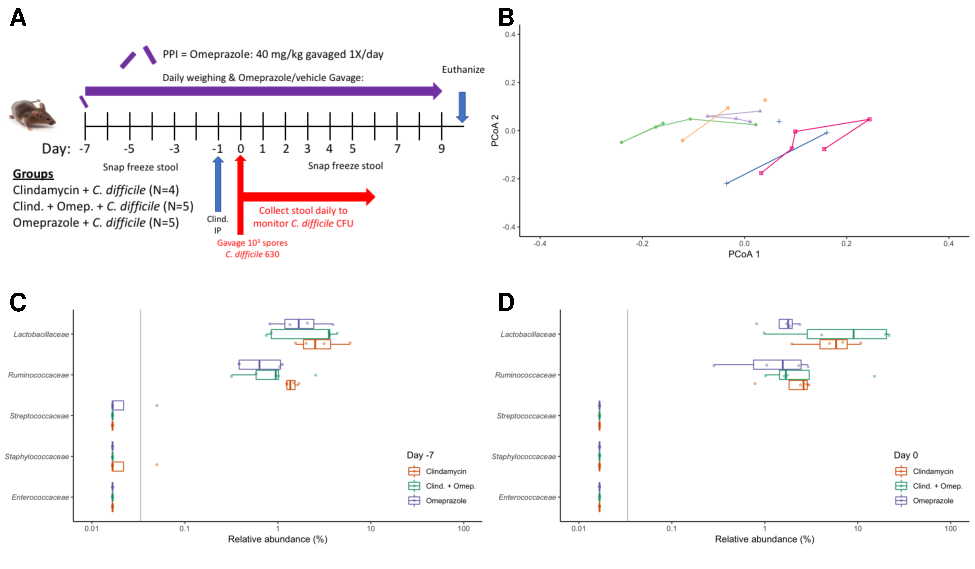
\includegraphics{figure_1.pdf} \textbf{Figure 1. Omeprazole treatment
had minimal impact on the murine fecal microbiota.} A. Mouse experiment
timeline and logistics. The PPI omeprazole was administered throughout
the duration of the experiment. Clindamycin was administered 1 day
before \emph{C. difficile} challenge on Day 0. Stools for 16S rRNA
sequencing analysis were collected on the days that are labeled (Day -7,
-5, -3, -1, 0, 1, 2, 3, 4, 5, 7, 9). \emph{C. difficile} CFU in the
stool was quantified daily through 6 days post-infection by anaerobic
culture. B. Principal Coordinates Analaysis (PCoA) of Bray-curtis
distances from stool samples of mice in the omeprazole treatment group
during the intial 7 days of the experiment. Each color represents stool
samples from the same mouse and lines connect sequentially collected
samples. C-D. Relative abundances of families previously associated with
PPI use in humans at the start of the experiment (C) and after 7 days of
omeprazole treatment (D). Each circle represents an individual mouse.
There were no significant differences acoss treatment groups for any of
the identified families in the seqeunce data at day -7 and day 0,
analyzed by Kruskal-Wallis test with a Benjamini-Hochberg correction for
multiple comparisons. For C-D, the grey vertical line indicates the
limit of detection.

\newpage

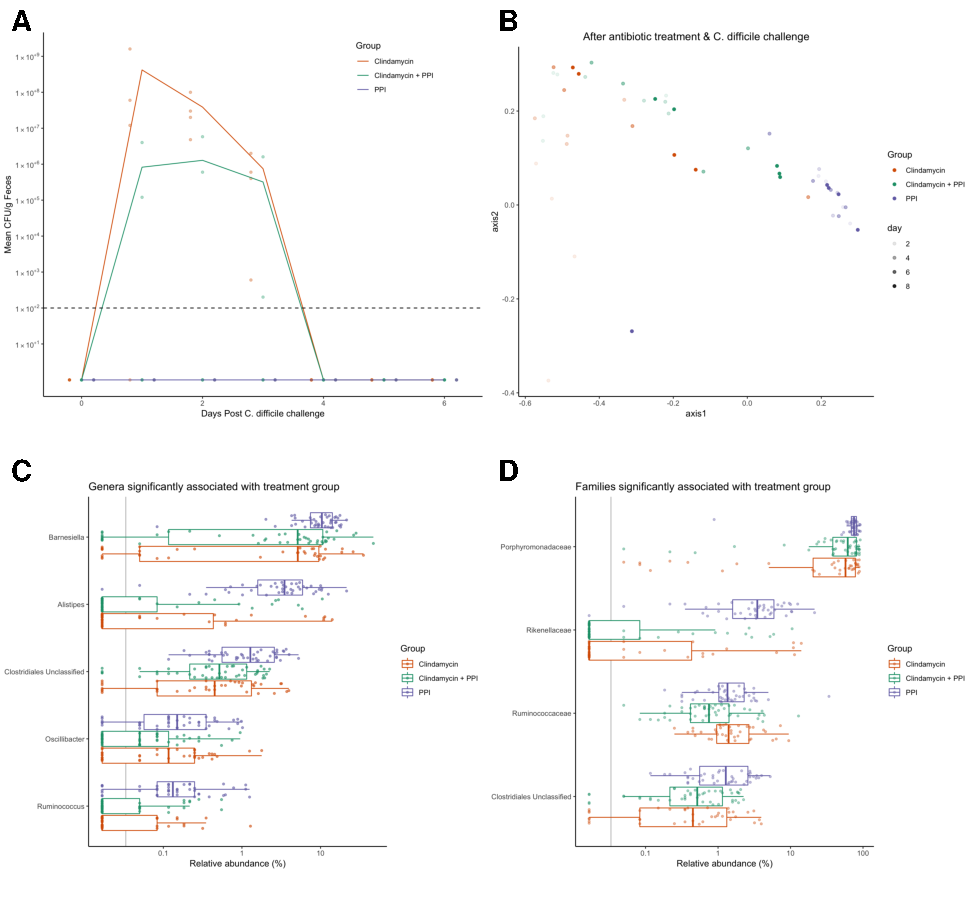
\includegraphics{figure_2.pdf} \textbf{Figure 2. Omeprazole treatment
alone does not promote CDIs in mice.} A. \emph{C. difficile} CFUs/g
stool measured each day post \emph{C. difficile} challenge for
clindamycin, clindamycin/PPI, and PPI-treated mice. Lines represent the
mean CFU/g for each treatment group while points represent CFU/g for
individual mice within each group. The black dashed line indicates the
limit of detection. B. PCoA of of Bray-curtis distances from stool
samples collected after antibiotic treatment (last 9 days of the
experiment). Transparency of the symbol corresponds to treatment day.
Symbols represent the \emph{C. difficile} colonization status of the
mice measured 2 days post-infection. Circles represent resistant mice
(\emph{C. difficile} was undetectable in stool samples), while X-shapes
represent mice that were colonized with \emph{C. difficile}, although
all mice cleared \emph{C. difficile} within 5 days of infection.
Omeprazole treated fecal samples primarily cluster together throughout
the experiment. C. Genera that vary the most across treatment groups for
stool samples collected from mice 2 days post-infection. Data were
analyzed by Kruskal-Wallis test, and no P values were significant after
Benjamini-Hochberg correction for multiple comparisons. The grey
vertical line indicates the limit of detection.

\newpage

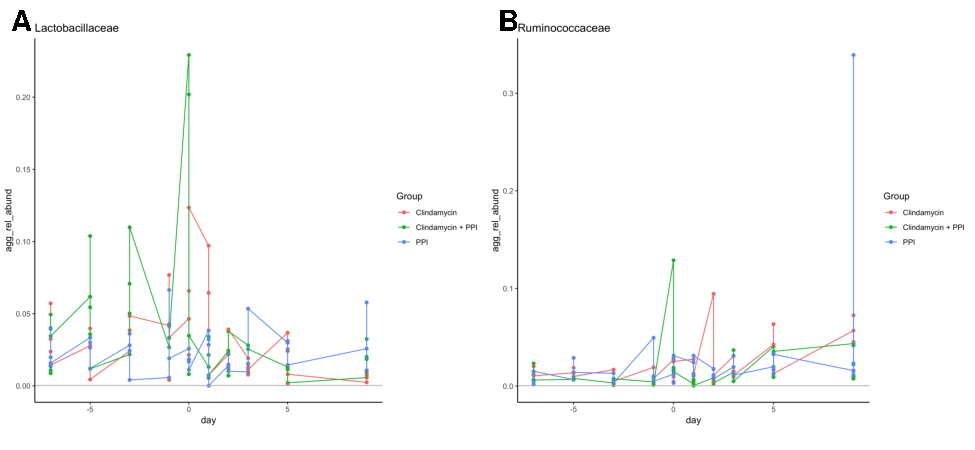
\includegraphics{figure_s1.pdf} \textbf{Figure S1. Families within
omeprazole treated mice fluctuate over time with no overall trend in
either direction.} Relative abundance over time for Lactobacillaceae (A)
and Ruminococcaceae (B), 2 of the PPI-associated familes from human PPI
studies across all 3 treatment groups. Each point represents the
relative abundance for an individual mouse stool sample, while the lines
represent the mean relative abundances for each treatment group of mice.
The grey horizontal lines indicate the limit of detection.

\newpage

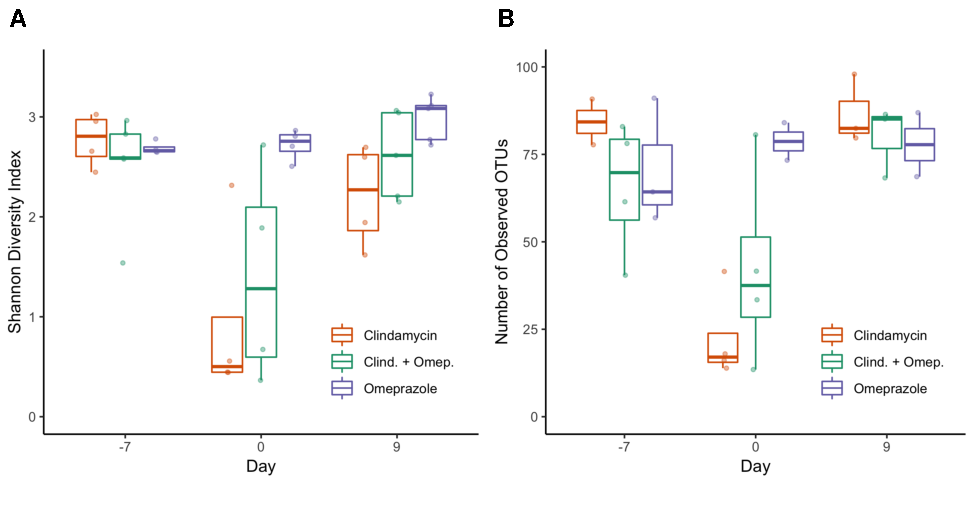
\includegraphics{figure_s2.pdf} \textbf{Figure S2. Microbiota diversity
and richness decrease with antibiotic treatment but remain relatively
constant with omeprazole treatment.} A. Boxplots of the Shannon
Diversity Index values (A) and number of observed OTUs (B) for each
group of mice over 3 timepoints (Day -7, 0, and 9). Each circle
represents the value for a stool sample from an individual mouse.


\end{document}
